\subsection{Blockchain}

\subsubsection{Costos}

\paragraph{Swarm}
Al deployar el sitio web es necesario contar con \textit{postage stamps} que son la manera de pagar por el uso del almacenamiento en Swarm. Cada actualización que se realice al sitio requiere de \textit{postage stamps} y, además, estos tienen fecha de vencimiento por lo que es necesario volver a pagar frecuentemente. Dichos \textit{postage stamps} se pagan en la criptomoneda BZZ que fluctúa de valor con respecto al dólar estadounidense. La obtención del sitio web no requiere de costo alguno, por lo que desde el punto de vista de un usuario lector de la aplicación no sería necesario pagar.

El valor de los \textit{stamps} también depende del tamaño del contenido a ser desplegado y el tiempo que se quiere mantener el contenido en la red, esto lo manejan con variables llamadas \textit{depth} y \textit{amount} que uno puede variar para obtener el almacenamiento y tiempo requerido. Realizando un despliegue desde un nodo de Swarm que apunta a la testnet Sepolia, un \textit{postage stamp} con 1GB de almacenamiento por 2 días (\textit{depth} 20 y \textit{amount} 10000000000) tiene un costo de 1.0486 BZZ que equivalen a 0.1767 USD (al día 11/06/2025).

\paragraph{Ethereum}
Se utiliza la moneda ETH para pagar por cada transacción, esto incluye tanto el despliegue de cada \textit{smart contract} como también cada modificación al estado de los mismos. Por lo tanto, el usuario final de la aplicación termina pagando por la creación y edición de cada artículo en el repositorio de conocimiento, y por cada mensaje enviado en el mensajero en tiempo real. Por otro lado, para las operaciones de lectura no se tiene que pagar nada. A este monto que tiene que pagar el usuario se lo llama gas y varía con respecto a las operaciones que realiza el método que se ejecuta al llamar a un \textit{smart contract} y, también, con respecto a la congestión de la red, es decir a mayor congestión mayor será el costo.

\begin{figure}[H]
    \centering
    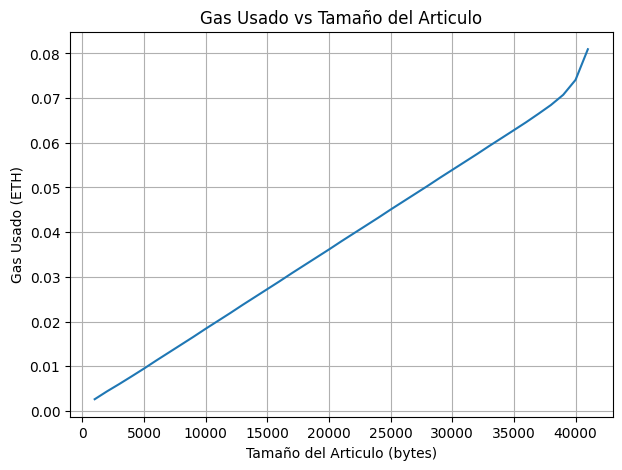
\includegraphics[width=0.75\linewidth]{img/aw-eth-bytes-articulo-incremental-gas.png}
    \caption{Gas usado al crear artículos con tamaño de bytes creciente}
    \label{fig:aw-eth-bytes-articulo-incremental-gas}
\end{figure}

\subsubsection{Experiencia de desarrollo} % Developer Experience

\paragraph{Swarm}
La experiencia de desarrollo en Swarm podría ser mejor. Cuenta con una comunidad pequeña pero activa. Si bien la documentación en varios aspectos puede resultar escasa, tienen medios por los cuales se pueden consultar dudas al equipo de desarrollo y son respondidas con brevedad.

Existen algunas herramientas que facilitan el desarrollo, por ejemplo, swarm-cli \cite{swarm-cli} la cual permite la interacción con un nodo de Swarm para realizar despliegues o consultas sobre su estado. También el equipo de Swarm provee una Github Action que permite la posibilidad de automatizar el despliegue generando un pipeline que utilice dicha herramienta.

En cuanto a un ambiente de pruebas o \textit{staging}, si bien no existe un \textit{gateway} público que interactúe con la \textit{testnet}, es posible levantar uno propio que sí lo haga apuntando a la \textit{testnet} de Sepolia usando la herramienta gateway-proxy \cite{gateway-proxy}.

\paragraph{Ethereum}
La experiencia de desarrollo en Ethereum resulta positiva por su gran comunidad y herramientas que provee. Por ejemplo, con la librería web3.js se puede interactuar con un nodo de Ethereum y realizar un despliegue de la aplicación. Además, con las herramientas de Hardhat se puede levantar una red de prueba que facilita el desarrollo local. Por otro lado, cuenta con una extensa documentación que detalla el funcionamiento de su blockchain.

\subsubsection{Aplicabilidad al caso de uso}

\paragraph{Swarm}
Resulta más conveniente para sitios web o recursos estáticos, al igual que IPFS. Por otro lado, al ser una tecnología de almacenamiento no es posible la ejecución de código.

A diferencia de IPFS, Swarm cuenta con incentivos incluidos (por medio de la moneda BZZ), esto significa que para deployar contenido en la red es necesario pagar. Al hacerlo te asegura que el mismo va a estar disponible durante el tiempo equivalente al costo pagado, es decir, que no es necesario pinear los archivos puesto que se encuentran en la red con un TTL.

\paragraph{Ethereum}
Su punto fuerte es la ejecución de código, por lo cual es útil para funcionar como backend de aplicaciones web. Como hemos visto, por el costo de almacenamiento de los smart contracts, no es recomendable para recursos como imágenes, videos o incluso strings de texto muy largos como lo realizado en el repositorio de conocimiento. 

Los eventos pueden resultar útil para la interacción en tiempo real requerida en el mensajero, pero lo positivo de esto queda opacado por el hecho de necesitar pagar por cada interacción, en el caso del mensajero por cada mensaje enviado. Esto se puede volver costoso rápidamente, además de tedioso al momento de utilizar la aplicación. Se pueden explorar alternativas para reducir esta fricción, como por ejemplo, que el contrato tenga un balance de tokens para ser gastados, lo cual haría que el usuario no tenga que confirmar cada transacción de mensaje enviado si no que directamente el contrato lo extrae de su balance; entre otras posibilidades.

\subsubsection{Performance\label{performance-blockchain}}

Para el caso del sitio web estático las métricas obtenidas se realizaron mediante un nodo local apuntando a la testnet Sepolia. Los valores son una aproximación a lo que sería en la mainnet. Para el caso de la mainnet habría que tener en cuenta que el tiempo de red puede ser mayor.

Las métricas para el repositorio de conocimiento y para el mensajero en tiempo real se obtuvieron levantando una instancia local de Hardhat \cite{hardhat}. Los tiempos obtenidos corresponden al que le toma a la transacción ejecutarse en una máquina local. En un caso real, existe un tiempo mayor de red y de interacción del usuario con la \textit{wallet} para confirmar la transacción.

\paragraph{Sitio Web Estático}

\subparagraph{Despliegue de contenido}

Al realizar el despliegue de sitios con distintas cantidades de archivos y tamaños se obtuvieron los resultados de la Tabla \ref{table:estadisticas-despliegue-swarm}. Vemos que la cantidad de archivos no tiene un efecto en el tiempo de publicación del contenido mientras el tamaño total del sitio se mantenga igual.

\setlength\tabcolsep{10pt}
\begin{table}[H]
    \centering
    \begin{tabular}{|c|c|c|c|c|c|}
    \hline
    & \textbf{Max} & \textbf{Mean} & \textbf{Min} & \textbf{Std} & \textbf{Median} \\
    \hline
    \textbf{1KiB-50files} & 13.93 s & 8.95 s & 5.24 s & 1.74 s & 8.83 s \\
    \hline
    \textbf{25KiB-50files} & 9.92 s & 7.99 s & 5.81 s & 1.19 s & 8.38 s \\
    \hline
    \textbf{50KiB-1files} & 10.39 s & 7.65 s & 5.75 s & 1.13 s & 7.79 s \\
    \hline
    \textbf{50KiB-10files} & 22.65 s & 8.84 s & 5.49 s & 3.73 s & 7.59 s \\
    \hline
    \textbf{50KiB-25files} & 10.41 s & 8.20 s & 5.66 s & 1.18 s & 8.24 s \\
    \hline
    \textbf{50KiB-50files} & 14.59 s & 8.62 s & 5.36 s & 1.80 s & 8.52 s \\
    \hline
    \end{tabular}
    \caption{Estadísticas para desplegar contenido en Swarm}
    \label{table:estadisticas-despliegue-swarm}
\end{table}

\paragraph{Repositorio de conocimiento}

\subparagraph{Tiempo en obtener un artículo}

En la siguiente tabla podemos ver los resultados de obtener 1000 muestras de la obtención de un mismo artículo en los distintos tamaños. No se nota diferencia significativa entre los tamaños \textit{short} y \textit{medium}, pero sí se puede ver un salto en la latencia al obtener un artículo de tamaño \textit{large}.

\setlength\tabcolsep{10pt}
\begin{table}[!htbp]
    \centering
    \begin{tabular}{|c|c|c|c|c|c|}
    \hline
    & \textbf{Max} & \textbf{Mean} & \textbf{Min} & \textbf{Std} & \textbf{Median} \\
    \hline
    \textbf{short} & 42.03 ms & 11.26 ms & 6.44 ms & 3.28 ms & 10.51 ms \\
    \hline
    \textbf{medium} & 33.35 ms & 15.30 ms & 9.11 ms & 3.47 ms & 14.66 ms \\
    \hline
    \textbf{large} & 135.32 ms & 47.46 ms & 31.05 ms & 7.82 ms & 46.34 ms \\
    \hline
    \end{tabular}
    \caption{Tiempo en obtener un artículo}
\end{table}

\subparagraph{Tiempo de creación de artículos}

Se registró el tiempo de creación de un artículo aumentando el tamaño en bytes del mismo. La Figura \ref{fig:aw-eth-bytes-articulo-incremental-tiempo} muestra el resultado de tomar el promedio de 5 muestras por tamaño de artículo, aumentando el mismo de a 1000 bytes por iteración.

\begin{figure}[H]
    \centering
    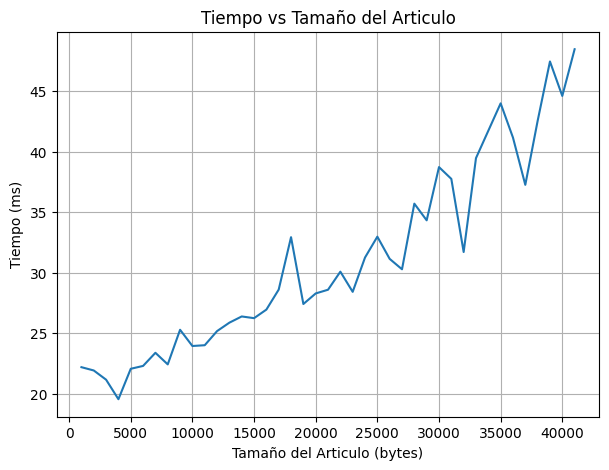
\includegraphics[width=0.75\linewidth]{img/aw-eth-bytes-articulo-incremental-tiempo.png}
    \caption{Tiempo para crear artículos con tamaño de bytes creciente}
    \label{fig:aw-eth-bytes-articulo-incremental-tiempo}
\end{figure}

\textbf{Mensajero en tiempo real}\\

Las siguientes métricas se obtuvieron levantando una instancia local de Hardhat \cite{hardhat} y ejecutando 850 muestras y 3 veces cada una.

\subparagraph{Tiempo en enviar un mensaje}

La primer métrica tomada corresponde al tiempo que tarda en enviarse un mensaje.

\setlength\tabcolsep{10pt}
\begin{table}[!htbp]
    \centering
    \begin{tabular}{|c|c|c|c|c|c|}
    \hline
    & \textbf{Max} & \textbf{Mean} & \textbf{Min} & \textbf{Std} & \textbf{Median} \\
    \hline
    \textbf{short} & 10.93 ms & 6.12 ms & 5.09 ms & 0.74 ms & 6.01 ms \\
    \hline
    \textbf{medium} & 10.34 ms & 6.26 ms & 5.24 ms & 0.60 ms & 6.20 ms \\
    \hline
    \textbf{large} & 10.68 ms & 6.44 ms & 5.36 ms & 0.70 ms & 6.37 ms \\
    \hline
    \end{tabular}
    \caption{Tiempo en enviar un mensaje}
\end{table}

Se puede observar que los tiempos entre los tamaños de mensajes no varían demasiado.

\subparagraph{Gas usado para enviar un mensaje}

La siguiente tabla muestra el valor (en ETH y USD) de enviar el mismo mensaje corto. El precio tomado para la conversión de ETH a dólar es el de la fecha del 5 de junio de 2025 a las 19:00hs de \$2439.17 de la página \href{https://coinmarketcap.com/currencies/ethereum/}{Coinmarketcap}.

\setlength\tabcolsep{10pt}
\begin{table}[H]
    \centering
    \begin{tabular}{|c|c|c|c|c|c|c|}
    \hline
    & & \textbf{Max} & \textbf{Mean} & \textbf{Min} & \textbf{Std} & \textbf{Median} \\
    \hline
    \multirow{2}{*}{\textbf{short}} & \textbf{ETH} & 0.00042043 & 0.00034257 & 0.00034221 & 0.00000331 & 0.00034221 \\
    \cline{2-7}
    & \textbf{USD} & 1.03 & 0.84 & 0.83 & 0.01 & 0.83 \\
    \hline
    \multirow{2}{*}{\textbf{medium}} & \textbf{ETH} & 0.00060668 & 0.00051325 & 0.00051274 & 0.00000434 & 0.00051274 \\
    \cline{2-7}
    & \textbf{USD} & 1.48 & 1.25 & 1.25 & 0.01 & 1.25 \\
    \hline
    \multirow{2}{*}{\textbf{large}} & \textbf{ETH} & 0.00085774 & 0.00074335 & 0.00074264 & 0.00000579 & 0.00074264 \\
    \cline{2-7}
    & \textbf{USD} & 2.09 & 1.81 & 1.81 & 0.01 & 1.81 \\
    \hline
    \end{tabular}
    \caption{Precio y gas usado para enviar un mensaje}
\end{table}

Según los resultados obtenidos se puede decir que para enviar un mensaje cuesta más de 1 dólar.

\subparagraph{Tiempo en obtener mensajes}

Para esta métrica se tomó el tiempo en obtener todos los mensajes para un chat el cual iba teniendo cada vez más mensajes (desde 0 hasta 850 mensajes). El gráfico muestra para los 3 tipos de mensajes, cómo el tiempo (en milisegundos) se va incrementando a medida que hay más mensajes en el chat.

\begin{figure}[H]
    \centering
    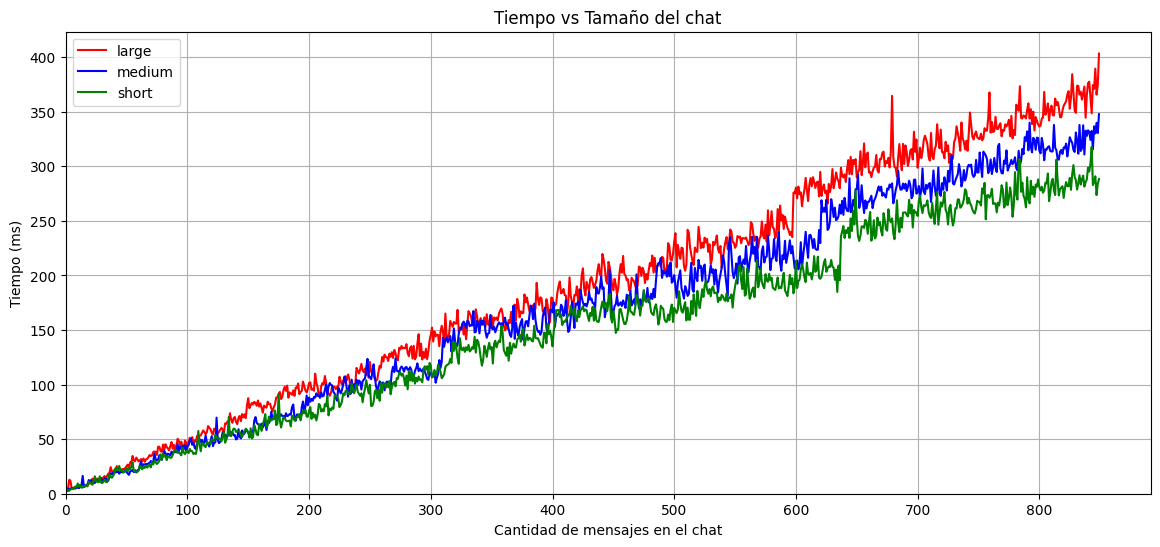
\includegraphics[width=1\linewidth]{img/blockchain-get-message-graphic.png}
    \caption{Tiempo para obtener mensajes de un chat según el tamaño del chat}
    \label{fig:blockchain-get-message-graphic.png}
\end{figure}

\subparagraph{Tiempo entre enviar y recibir un mensaje (mismo usuario)}

En esta métrica se midió el tiempo que tarda en un mensaje desde que es enviado a ser recibido por el canal de escucha de nuevos mensajes para un mismo usuario.

\setlength\tabcolsep{10pt}
\begin{table}[H]
    \centering
    \begin{tabular}{|c|c|c|c|c|c|}
    \hline
    & \textbf{Max} & \textbf{Mean} & \textbf{Min} & \textbf{Std} & \textbf{Median} \\
    \hline
    \textbf{short} & 38.12 ms & 5.42 ms & 4.26 ms & 1.62 ms & 4.66 ms \\
    \hline
    \textbf{medium} & 28.97 ms & 5.76 ms & 4.31 ms & 1.74 ms & 5.05 ms \\
    \hline
    \textbf{large} & 24.66 ms & 5.76 ms & 4.46 ms & 0.94 ms & 5.6 ms \\
    \hline
    \end{tabular}
    \caption{Tiempo en enviar y recibir un mensaje (mismo usuario)}
    \label{tab:tiempo-send-recv-same-user}
\end{table}

\subparagraph{Tiempo entre enviar y recibir un mensaje (distintos usuarios)}

Esta métrica calcula el tiempo que tarda un segundo usuario en recibir un mensaje enviado por un primer usuario.

\setlength\tabcolsep{10pt}
\begin{table}[H]
    \centering
    \begin{tabular}{|c|c|c|c|c|c|}
    \hline
    & \textbf{Max} & \textbf{Mean} & \textbf{Min} & \textbf{Std} & \textbf{Median} \\
    \hline
    \textbf{short} & 13.19 ms & 5.61 ms & 4.59 ms & 0.97 ms & 5.53 ms \\
    \hline
    \textbf{medium} & 10.92 ms & 5.84 ms & 4.53 ms & 1.28 ms & 5.06 ms \\
    \hline
    \textbf{large} & 13.95 ms & 5.96 ms & 4.65 ms & 0.72 ms & 5.89 ms \\
    \hline
    \end{tabular}
    \caption{Tiempo en enviar y recibir un mensaje (distintos usuarios)}
    \label{tab:tiempo-send-recv-diff-user}
\end{table}

Si comparamos las tablas de tiempos de enviar y recibir un mensaje (\ref{tab:tiempo-send-recv-same-user} y \ref{tab:tiempo-send-recv-diff-user}) vemos que los tiempos son parecidos. Si bien los máximos de la primer tabla son mayores que los de la segunda y los datos están más dispersos, para los demás valores de la segunda tabla estos tienden a ser ligeramente mayores. En este caso particular, si se hiciera una prueba entre 2 usuarios de distintas partes del mundo el tiempo de conexión seguramente pesaría más.

\subsubsection{Sistema utilizado}

Para realizar las métricas del sitio web estático y el repositorio de conocimiento en Blockchain, se utilizó el siguiente sistema:
\begin{itemize}
    \item \textbf{CPU:} Ryzen 5 1600
    \item \textbf{RAM:} 16GB
    \item \textbf{Almacenamiento:} SSD
\end{itemize}

En cuanto al mensajero en tiempo real, las especificaciones del sistema en el cual se realizaron las métricas son las siguientes:

\begin{itemize}
    \item \textbf{CPU:} Ryzen 7 5700X
    \item \textbf{RAM:} 32GB
    \item \textbf{Almacenamiento:} HDD
\end{itemize}